%% Esempio per lo stile supsi
\documentclass[twoside]{supsistudent} 

\usepackage{listings}
% per settare noindent
\setlength{\parindent}{0pt}


\usepackage{color}

\definecolor{mygreen}{rgb}{0,0.6,0}
\definecolor{mygray}{rgb}{0.5,0.5,0.5}
\definecolor{mymauve}{rgb}{0.58,0,0.82}

\lstset{ 
  backgroundcolor=\color{white},   % choose the background color; you must add \usepackage{color} or \usepackage{xcolor}; should come as last argument
  basicstyle=\footnotesize,        % the size of the fonts that are used for the code
  breakatwhitespace=false,         % sets if automatic breaks should only happen at whitespace
  breaklines=true,                 % sets automatic line breaking
  captionpos=b,                    % sets the caption-position to bottom
  commentstyle=\color{mygreen},    % comment style
  deletekeywords={...},            % if you want to delete keywords from the given language
  escapeinside={\%*}{*)},          % if you want to add LaTeX within your code
  extendedchars=true,              % lets you use non-ASCII characters; for 8-bits encodings only, does not work with UTF-8
  frame=single,	                   % adds a frame around the code
  keepspaces=true,                 % keeps spaces in text, useful for keeping indentation of code (possibly needs columns=flexible)
  keywordstyle=\color{blue},       % keyword style
  language=Octave,                 % the language of the code
  morekeywords={*,...},            % if you want to add more keywords to the set
  numbers=left,                    % where to put the line-numbers; possible values are (none, left, right)
  numbersep=5pt,                   % how far the line-numbers are from the code
  numberstyle=\tiny\color{mygray}, % the style that is used for the line-numbers
  rulecolor=\color{black},         % if not set, the frame-color may be changed on line-breaks within not-black text (e.g. comments (green here))
  showspaces=false,                % show spaces everywhere adding particular underscores; it overrides 'showstringspaces'
  showstringspaces=false,          % underline spaces within strings only
  showtabs=false,                  % show tabs within strings adding particular underscores
  stepnumber=2,                    % the step between two line-numbers. If it's 1, each line will be numbered
  stringstyle=\color{mymauve},     % string literal style
  tabsize=2,	                   % sets default tabsize to 2 spaces
  title=\lstname                   % show the filename of files included with \lstinputlisting; also try caption instead of title
}



% Crea un capitolo senza numerazione che pero` appare nell'indice %
\newcommand{\problemchapter}[1]{%
  \chapter*{#1}%
  \addcontentsline{toc}{chapter}{#1}%
\markboth{#1}{#1}
}

% Numerazione delle appendici secondo norma
\addto\appendix{
\renewcommand{\thesection}{\Alph{chapter}.\arabic{section}}
\renewcommand{\thesubsection}{\thesection.\arabic{subsection}}}

% Crea una sezione senza numerazione che pero` appare nell'indice %
\newcommand{\problemsection}[1]{%
  \section*{#1}%
  \addcontentsline{toc}{section}{#1}%
\markboth{#1}{#1}
}

%----------------------------------------------------------------
%Definizione comandi
%----------------------------------------------------------------
\renewcommand{\contentsname}{Indice\vspace{5mm}}
\newcommand{\DecaTitolo}{Laboratorio - sviluppo applicazioni web}
\newcommand{\Decaa}{\newline\vspace{0.5mm}\newline\noindent}

\setcounter{secnumdepth}{5} 	%per avere più livelli nei titoli
\setcounter{tocdepth}{5}		%per avere più livelli nell'indice

\titolo{Progetto semestre: Libreria di supporto per riconoscimento immagini}
\studente{Andrea De Carlo \vspace{1em}\\ Roberto Trapletti }
\relatore{Giacomo Poretti}
\correlatore{}
\committente{DSwiss}
\corso{Ingegneria Informatica}
\modulo{M02042P}
\anno{2018/2019}

\begin{document}

\pagenumbering{alph}
\maketitle
\onehalfspacing
\frontmatter


\pagenumbering{roman}
\tableofcontents
% \listoffigures					% Opzionale
% \listoftables					% Opzionale


\problemchapter{Abstract} %rob
\problemsection{Abstract italiano}
Il progetto affronta come prima parte un problema di riconoscimento immagini utilizzando tecnologie mobile. L’obiettivo della libreria è quello di fornire le funzioni di supporto da utilizzare successivamente con un’applicazione di salvataggio password e documenti. Si vuole facilitarne il recupero permettendo all’utente di eseguire una ricerca tramite foto.
La seconda parte è un’analisi esplorativa delle tecnologie in ambito di Machine Learning utilizzabili a livello mobile. Per capire quali metodi sono usati attualmente e come funzionano, nella libreria è utilizzato un classificatore per aumentarne la robustezza, determinando se nell’immagine scattata dall’utente è presente uno schermo. 
\problemsection{Abstract inglese}
In the first part of this project, we deal with a problem of image recognition using mobile technologies.. The purpose of the library is to provide the support functions to be used later with an application that save passwords and documents. The goal is to facilitate recovery of the access keys by allowing the user to search through photos.
The second part is an exploratory analysis of the technologies in Machine Learning that can be used on a mobile. To understand which methods are currently used and how they work, a classifier is used in the library to increase its robustness, determining if a screen is present in the image taken by the user.


\problemchapter{Progetto assegnato} %rob
\problemsection{Descrizione}
Scopo del progetto è quello di rilevare tramite smartphone indirizzi (URL) o codici particolari testuali (per esempio password) visualizzati su uno schermo, per esempio di un PC.

Si tratta quindi di realizzare un programma per smartphone Android che tramite funzioni di Computer Vision sia in grado di riconoscere dei caratteri (OCR) in determinate zone dello schermo.

Il progetto è realizzato su richiesta della ditta DSwiss che fornirà dettagli supplementari e seguirà il progetto per requisiti e verifiche dei risultati ottenuti.

\problemsection{Compiti}
\begin{itemize}
\item Sviluppare un'applicazione Android
\item Riconoscere uno schermo
\item Estrarre i caratteri visualizzati sullo schermo
\item Isolare URL da indirizzi o codici esposti in zona precisa schermo
\end{itemize}

\problemsection{Tecnologie}
Java, Android, OpenCV per Android o altri framework particolari di OCR disposnibili per Android

\newpage
\mainmatter
\pagenumbering{arabic}
\setcounter{page}{1}



\chapter{Introduzione}
\section{Contesto del progetto}
    %dire che per la ditta è importante un concetto di intelligenza artificiale
    La ditta committente DSwiss dispone di una applicazione sia client che mobile di gestione delle password. Nello stato attuale, queste password vengono salvate all'interno di un DB locale sempre a disposizione dell'utente.
    \Decaa
    Hanno pensato di aggiungere una nuova caratteristica, ovvero un sistema di ricerca automatica della password da inserire, tramite una fotografia della pagina di login.
    Vorrebbero quindi applicare delle tecnologie ingegneristiche di computer vision per comprendere da una immagine appena scattata, il dominio della pagina web (sito) e recuperarne la password associata.
    \Decaa
    Ulteriormente all'incarico commissionato, la ditta in questione ha suscitato dell'interesse importante per il concetto di intelligenza artificiale. Andremo quindi ad eseguire una analisi esplorativa dei concetti base di machine learning in ambito PC e mobile.
    
\section{Evoluzione e adattamento degli obbiettivi}
\subsection{Preambolo}
\subsection{Obbiettivi iniziali della richiesta}
Durante l’assegnazione dei lavori di semestre, per questo progetto erano stati prefissati i seguenti obbiettivi:

\begin{itemize}
\item Sviluppare un'applicazione Android
\item Riconoscere uno schermo
\item Estrarre i caratteri visualizzati sullo schermo
\item Isolare URL da indirizzi o codici esposti in zona precisa schermo
\end{itemize}

Durante un primo incontro con il committente, abbiamo scoperto che questi obbiettivi non erano confacenti alla effettiva richiesta esposta dalla ditta. Abbiamo pertanto stilato, con l’aiuto del relatore e del committente, una nuova lista degli obbiettivi.

% METTERE GLI OBBIETTIVI NUOVI IN MANIERA POLITICALLY CORRECT
\begin{itemize}
\item Sviluppare un concetto di libreria per android
\item Riconoscere uno schermo
\item Ritornare il dominio di un sito data una fotografia
\end{itemize}

\chapter{Requisiti e specifiche} 
Il requisito più importante e limitante a livello di programmazione è quello che tutta la libreria deve utilizzare solo ed unicamente le risorse locali dei dispositivi mobile, per questioni di sicurezza. Questo significa che i servizi come le API Vision di Google, le API Computer Vision di Azure della Microsoft o Amazon Rekognition di Amazon, non sono utilizzabili.  

\chapter{Fase analitica}
\section{Stato dell'arte} %rob
\subsection{Feature detection}%rob
Quando giochiamo con i puzzle, il nostro cervello esegue due operazioni significative: determina quali punti di un singolo pezzo sono importanti, che quindi possano essere comparati facilmente, e cerca di descriverli, in modo da trovare collegamenti con gli altri pezzi. In computer vision eseguire una feature detection significa ricercare quali punti possono essere utilizzati per una comparazione. Esistono diversi algoritmi che si possono basare su: \begin{itemize}
\item Contorni, bordi
\item Angoli
\item Regioni
\item Creste
\end{itemize}
Una volta trovati questi punti bisogna anche trovare il modo più efficiente per descriverli. Per questo esistono altri tipi di algoritmi chiamati "algoritmi di feature description"
Una volta ottenute i punti d'interesse e la loro descrizione si possono cercare le stesse feature in altre immagini e quindi determinare la presenza di corrispondenze. 
Gli algoritmi più conosciuti sono:
\begin{itemize}
\item SIFT
\item SURF
\item BRIEF
\item KAZE
\end{itemize}
La libreria più utilizzata in questo ambito è OpenCV. È una libreria sotto 3-clause BSD License. Esiste il supporto per Python, Java e C++ e anche qualche binding di terze parti. Contiene delle implementazioni ottimizzate per la maggior parte dei comuni algoritmi e tecniche utilizzate in computer vision.
L'algoritmo che abbiamo potuto testare più performante è senz'altro il SURF. Purtroppo è un algoritmo patentato e l'utilizzo ne richiede quindi una licenza apposita. Nei nostri progetti di test mobile abbiamo utilizzato il KAZE che richiede un po' più di tempo.
\subsubsection{Feature detection su smartphone}%rob
La libreria OpenCV ha un porting per Android e anche per IOS. Per lo sviluppo con strumenti pensati per il multiplatform, come Xamarin, esistono delle librerie di terza parti. La ditta DSwiss utilizza come strumento di sviluppo proprio Xamarin, per questo motivo abbiamo cercato librerie disponibili in quest'ambito. Abbiamo scoperto Accord.NET, che in teoria offre funzionalità di Machine Learning, di image processing, di computer vision e molto altro. Ha una versione leggera pensata per i dispositivi mobili. Altro punto positivo è la licenza: GNU Lesser Public License v2.1. Purtroppo, abbiamo provato a utilizzarla senza successo, dato che gli sviluppatori sono ancora ad una versione alpha e il build non funziona in determinate condizioni. Per questo motivo nella nostra libreria abbiamo utilizzato EMGU.CV. È un wrapper .NET di OpenCV. Dispone di due modelli di licenza, una open source (GNU GPL license v3) o commerciale. Alcune funzionalità sono disponibili solo utilizzando la licenza commerciale. A scopo di test e didattico abbiamo chiesto e ricevuto una versione di prova della libreria completa. 
\subsection{Machine learning}%rob
\begin{quote}
    «Si dice che un programma apprende dall’esperienza E con riferimento a alcune classi di compiti T e con misurazione della performance P, se le sue performance nel compito T, come misurato da P, migliorano con l’esperienza E».
\end{quote}
    In pratica le tecniche di Machine Learning permettono ai computer di imparare dall'esperienza. ML si può suddividere in tre principali categorie: l'apprendimento supervisionato, l'apprendimento non supervisionato e l'apprendimento per rinforzo. La scelta del tipo di apprendimento da utilizzare dipende naturalmente dal problema da risolvere e dalla capacità computazionale del dispositivo che utilizzeremo. 
    L'apprendimento supervisionato consiste nel fornire ad un sistema un dataset di informazioni in input e il releativo risultato. Per affrontare il suo compito il computer analizza il dataset e cerca di trovare delle regole in base a quanto già visto. La risposta che fornirà sarà quella più probabile secondo le sue esperienze, quindi secondo i dati passati in ingresso. 
    L'addestramento non supervisionato differisce da quello supervisionato perché le informazioni che inseriamo all'inizio non sono classificate, i risultati non esistono. Il computer stesso deve definire le caratteristiche di una classe. Viene utilizzato in problemi di clustering, cioè il raggruppare in diversi insieme determinati elementi.
    L'apprendimento per rinforzo è utilizzato in ambienti dinamici dove il computer deve raggiungere un obbiettivo. Si utilizza un sistema di ricompense e penalità. L'esempio più comune è l'utilizzo nelle auto senza pilota. 
    
    \subsubsection{Deep learning e Neural network}
    Nella nostra libreria utilizzeremo il deep learning per renderla più robusta e per determinare se ci sono e quali loghi in una determinata immagine. Il deep learning è una sotto categoria del machine learning ed consiste nel produrre modelli di apprendimento su più livelli. 
    In generale impara nuove nozioni da ciò che impara nei livelli precedenti. Pensate ad un'immagine di un gatto. Dopo una prima analisi dell'immagine determina che ci sono, occhi, baffi, pelo, ecc... Al prossimo livello grazie alle informazioni raccolte in precedenza capisce che si tratta di un gatto. Potremmo anche aggiungere un ulteriore livello e capire di quale razza si tratta. Il deep learning ha fatto grandi passi negli ultimi anni grazie anche alla reperibilità sempre maggiore di dataset di ogni tipo. Al centro del deep learning si trovano le neural network. 
    Le reti neurali sono principalmente dei modelli matematici, che permettono di produrre una risposta in uscita dato un determinato input.
Queste tipologie di modelli matematici sono composti da livelli di "neuroni" stratificati, ovvero dei componenti procedurali (di calcolo o statistica) che simulano lo stesso funzionamento di un neurone (nodo) e le relative sinapsi (collegamento tra nodi). Questi strati si suddividono in strati di input, strati nascosti e strato finale, come da immagine.

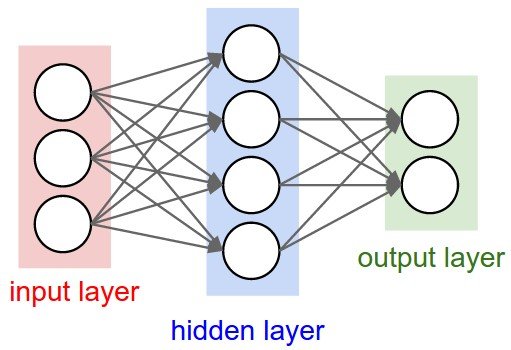
\includegraphics[width=\textwidth]{Pictures/neural_net.jpeg}

\subsubsection{Machine learning su smartphone}%rob
L'utilizzo del Machine Learning sui dispositivi mobili non è complicato. La parte che richiede più risorse computazionali infatti è la fase di training di un modello. Una volta ottenuto questo modello possiamo caricarlo nella nostra applicazione e utilizzarlo. I framework a disposizione sono molti, ma abbiamo avuto modo di testarne qualcuno come "ML .NET" che però sono risultati ancora non utilizzabili in termini di preparazione dell'ambiente di sviluppo e in termini di prestazioni. Tuttavia sono in fase di forte sviluppo, quindi ci aspettiamo un netto miglioramento di questo framework durante i prossimi mesi. Per la nostra libreria e i nostri test abbiamo provato quindi a utilizzare Tensorflow. Il test è avvenuto con successo sulla versione desktop mentre i binding della libreria presenti in Xamarin non funzionavano. Tensorflow però sta sviluppando un'alternativa per i dispositivi mobile chiamata Tensorflow Lite. Non abbiamo avuto modo di testarlo ma quello che abbiamo capito è che è meglio scrivere codice nativo senza passare da soluzioni multipiattaforma. Librerie cross-platfrom per Machine Learning e Computer Vision sono ancora troppo acerbe. 

\subsubsection{Dataset e modelli}%rob
Per il nostro progetto e per poter testare gli strumenti in ambito di Machine Learning abbiamo cercato di risolvere un problema di image recognition. Vogliamo verificare che in un'immagine sia presente o meno un monitor, uno schermo. Il primo passo per affrontare questo problema è trovare tante foto di monitor o schermi. In un primo momento abbiamo quindi optato per riaddestrare l'ultimo layer di una neural network già pronta. 
Per trovare molte immagini di monitor abbiamo utilizzato uno script python di un progetto git pubblico (vedi https://github.com/hardikvasa/google-images-download). Grazie a questo script si può eseguire il download di tot immagini da una ricerca in Google Immagini, specificandone anche il formato, la dimensione, ecc... Dopo aver scaricato le immagini le abbiamo processate per ridimensionarle tutte a 224x224 pixel. Questo perché addestrare l'ultimo layer di una neural network con immagini di dimensioni maggiori richiede più risorse e quindi di più tempo. Lo script è molto semplice:
\begin{lstlisting}[language=Python]
from PIL import Image
import os
import sys

directory = sys.argv[1]
saveDirectory = sys.argv[2]

for file_name in os.listdir(directory):
  print("Processing %s" % file_name)
  image = Image.open(os.path.join(directory, file_name))

  x,y = image.size
  new_dimensions = (224, 224)
  output = image.resize(new_dimensions, Image.ANTIALIAS)

  output_file_name = os.path.join(saveDirectory, file_name)
  output.save(output_file_name, "JPEG", quality = 95)

print("All done")
\end{lstlisting}

Dopo ulteriori ricerche tuttavia abbiamo recuperato un modello pre-addestrato per il riconoscimento immagini tra cui l'etichetta monitor o screen è presente nei nodi di output. Si chiama MobileNet ed è opensource. Si possono trovare differenti modelli (basati sullo stesso dataset ma addestrati in modo diverso) che differiscono per prestazioni, dimensioni e precisione.

\section{studio delle soluzioni - obiettivi iniziali}
Tenendo in considerazione gli obbiettivi iniziali di questo progetto,
\subsection{Decisione soluzione}
\section{studio delle soluzioni - obiettivi aggiuntivi}
\subsection{Decisione soluzione }

\chapter{design e concezione soluzioni}
\section{design soluzione obbiettivi iniziali}
\section{design soluzione obbiettivi aggiuntivi}

\chapter{implementazione soluzioni}%rob
\section{implementazione obbiettivi iniziali}%rob
Per lo sviluppo della nostra soluzione abbiamo pensato di creare un oggetto semplice, che abbiamo chiamato Record. L'idea è che questo oggetto contenga le informazioni ricavate da un esecuzione di un algoritmo di feature detection in modo che il processo di confronto con altre immagini non richieda troppe risorse. 

\begin{lstlisting}[language=C]

    [Serializable()]
    public class Record
    {
        ///////////////////////////////////////////////////////////
        ///Fields
        //////////////////////////////////////////////////////////

        private readonly String name;
        private readonly VectorOfKeyPoint keyPoint;
        private readonly Mat descriptors;

        public VectorOfKeyPoint KeyPoints { get { return keyPoint; } }
        public String Name { get { return name; } }
        public Mat Descriptors { get { return descriptors; } }

        // Private constructor
        private Record(String name) {
            this.name = name;
            this.keyPoint = new VectorOfKeyPoint();
            this.descriptors = new Mat();
        }
    ...
\end{lstlisting}

Questa classe espone un solo metodo:

\begin{lstlisting}[language=C]
public static Record CreateFromImage(String path, String name) {
            // new Record
            Record newRecord = new Record(name);

            //Preprocessing of the image
            Mat image = CvInvoke.Imread(path, ImreadModes.Color);
            UMat uImage = image.GetUMat(AccessType.Read);
            KAZE surf = new KAZE();
            surf.DetectAndCompute(uImage, null, newRecord.keyPoint, newRecord.descriptors, false);

            return newRecord;
        }
\end{lstlisting}

Come mostrato sopra, il metodo restituisce un nuovo record. Al Record è collegato una stringa "name" che serve a recuperare il valore corrispondente dell'immagine (come facebook, netflix, o anche l'URL direttamente, dipenderà da come vorrà essere utilizzata la libreria). Prima di restituire l'oggetto viene eseguito il metodo di feature detection e salvati i relativi dati. Questo metodo è pensato per ampliare il database locale qualora i dati precaricati non siano sufficienti o quando l'utente deve riconoscere siti personalizzati. 

La libreria vera e propria è la classe Reco.cs. Espone poche API atte a risolvere il problema proposto, come ad esempio il metodo per il recupero del nome data un'immagine in input. 

Attualmente date le tempistiche e lo scopo della libreria (conoscere quali strumenti si possono utilizzare per risolvere questo tipo di problemi) i Record sono serializzati e salvati localmente. Quando si utilizza la libreria si può richiamare un metodo load per caricare il file contenente i record in memoria. In futuro chiaramente si può migliorare questa gestione utilizzando ad esempio un componente come LINQ presente nel framework .NET.
Sono presenti due funzione per aggiunta e rimozione di record:


\begin{lstlisting}[language=C]
public bool AddImage(String imagePath, String name) {
            Record record;
            try
            {
                record = Record.CreateFromImage(imagePath, name);
                records.Add(record);
                return true;
            }
            catch (Exception e) {
                return false;
            }
            
        }
        
        /// <returns>Return true if the Record is found and correctly removed from the repository, else false</returns>
        public bool RemoveImage(String name) {
            return records.Remove(records.Find(r=>r.Name.Equals(name)));
        }
\end{lstlisting}

Abbiamo programmato un metodo chiamato GetNameList che, dato il percorso di un'immagine, genera un oggetto della classe Record, senza nessun nome associato, dopodichè utilizza le proprietà calcolate per generare un valore di score per ogni confronto. Sfruttando il metodo presente nella classe Utility, Sort List (che abbiamo implementato per ordinare la lista in base allo score di ogni confronto) restituisce una lista ordinata di coppie chiave-valore. La chiave è il nome registrato insieme al record mentre il valore rappresenta lo score risultante dalla comparazione. In questo modo si ottiene una lista di nomi per il quale il primo elemento è l'immagine con più punti in comune con quella in ingresso. 

Il sort è effettuato in questo modo:

\begin{lstlisting}[language=C]
  public static void sortList(List<KeyValuePair<string, int>> list) {
            list.Sort(
                delegate(KeyValuePair<string,int> pair1,
                KeyValuePair<string,int> pair2) {
                    return pair1.Value.CompareTo(pair2.Value);
                }
            );
          
        }
\end{lstlisting}

Il metodo invece si presenta così:

\begin{lstlisting}[language=C]
 private List<KeyValuePair<String, int>> GetNameList(String imagePath)
        {
            Record processingRecord = Record.CreateFromImage(imagePath, "");
            var resultList = new List<KeyValuePair<String, int>>();
            VectorOfVectorOfDMatch matches = new VectorOfVectorOfDMatch();
            int k = 2;
            double uniquenessThreshold = 0.8;
            Mat mask = new Mat();

            records.ForEach(e => {
                using (Emgu.CV.Flann.LinearIndexParams ip = new Emgu.CV.Flann.LinearIndexParams())
                using (Emgu.CV.Flann.SearchParams sp = new SearchParams())
                using (DescriptorMatcher matcher = new FlannBasedMatcher(ip, sp))
                {
                    matcher.Add(e.Descriptors);

                    matcher.KnnMatch(processingRecord.Descriptors, matches, k, null);
                    mask = new Mat(matches.Size, 1, DepthType.Cv8U, 1);
                    mask.SetTo(new MCvScalar(255));
                    Features2DToolbox.VoteForUniqueness(matches, uniquenessThreshold, mask);

                    // Calcluate the score based on matches size
                    int score = 0;
                    for (int i = 0; i < matches.Size; i++)
                    {
                        if (mask.GetData(i)[0] == 0) continue;
                        foreach (var item in matches[i].ToArray())
                            ++score;
                    }

                    // Add score and record's name to the map
                    resultList.Add(new KeyValuePair<string, int>(e.Name, score));
                }
            });

            Utility.sortList(resultList);
            return resultList;
        }
\end{lstlisting}
Per il confronto delle feature delle immagini esistono sono diverse possibilità. La prima soluzione è la più semplice ma naturalmente la meno efficace, si utilizza un Brute-Force Matcher. Prende in esame un descrittore di una feature della prima immagine e la confronta con il descrittore di ogni feature rilevata nella seconda. Calcola quindi una distanza utilizzando una determinata funzione e ritorna quella più vicina. Nella nostra libreria però noi abbiamo usato il FLANN Based Matcher. FLANN, acronimo di Fast Library for Approximate Nearest Neighbour, è una libreria contenente algoritmi di ricerca ottimizzati di nearest neighbour. In OpenCV, l'oggetto Flann Matcher riceve in ingresso due parametri, index\_params e search\_params. Il primo indica l'algoritmo da utilizzare e ne sono disponibili diversi, ognuno con le sue particolarità. La scelta dipende da quante risorse e quanto tempo si vuole dedicare a questa operazione. Il secondo parametro indica quante volte devono essere attraversati gli alberi nell'indice. Più volte significa più precisione ma naturalmente anche più tempo di elaborazione. 


\subsection{test e risultati}%rob


\section{implementazione obbiettivi aggiuntivi}%rob
\subsection{test e risultati}%rob

\chapter{Conclusioni}
\section{risultati ottenuti}
\subsection{obbiettivi raggiunti}
\subsection{obbiettivi non raggiunti}
\section{sviluppi futuri}%rob%rob
\section{competenze aquisite}%rob%rob

\chapter{Piano dei lavori}%rob%rob




%%% appendice %%%
% problemi riscontrati
% installazione ambienti di sviluppo
% installazione frameworks




%-------------------- Esempi da togliere -----------------------------------
% \chapter{Titolazione}

% \lipsum[13]

% \section{Sezione}

% \lipsum[23]
% Esempio di citazione \cite{4538384}, \cite{5357331,4523385}, \cite{1705631}.
% \footnote{Questa \`e una nota a pi\'e di pagina.}
% \footnote{Questa \`e un'altra nota a pi\'e di pagina.}
% \lipsum[23]

% \subsection{Sotto sezione}

% \texttt{Questo testo ha una spaziatura fissa}

% \textit{Questo testo \`e in italico}

% \textbf{Questo testo \`e in grassetto}

% \textsc{Questo testo \`e in maiuscoletto}

% \underline{Questo testo \`e sottolineato} \\

% Citazione:
% \begin{quote}
% \lipsum[23]
% \end{quote}

% \chapter{Titolazione}

% \lipsum[13]

% \begin{itemize}
%   \item Elemento A
%   \item Elemento B
%   \item Elemento C
% \end{itemize}

% %\begin{itemize}
% %  \item[-] Elemento A
% %  \item[-] Elemento B
% %  \item[-] Elemento C
% %\end{itemize}
% %
% %\begin{enumerate}
% %  \item Alpha
% %  \item Beta
% %  \item Gamma
% %\end{enumerate}

% \lipsum[23]
% %\section{Sezione}
% %
% %\lipsum[23]
% %
% %\subsection{Sotto sezione}
% %
% %Un po' di matematica: \newline
% %
% %\begin{math}
% %\frac{n!}{k!(n-k)!} = {n \choose k}
% %\end{math} \newline
% %
% %Un po' di matematica centrata:
% %
% %\begin{center}
% %\begin{math}
% %\frac{n!}{k!(n-k)!} = {n \choose k}
% %\end{math}
% %\end{center}
% %
% %Oppure con \$\$
% %
% %$$
% %\frac{n!}{k!(n-k)!} = {n \choose k}
% %$$
% %
% %Oppure anche direttamente nel testo ${1}\over{n}$ \\
% %
% %\lipsum[23]

\bibliographystyle{unsrt}
\bibliography{bibliografia}
\end{document}
